\section{MODELADO}
	Una vez se tienen los datos disponibles, se debe definir una arquitectura de entrenamiento de modelos de aprendizaje profundo sobre los datos, las redes neuronales se implementan en Python usando la libreria Pytorch.
	
	\begin{figure}[H]
		\centering
		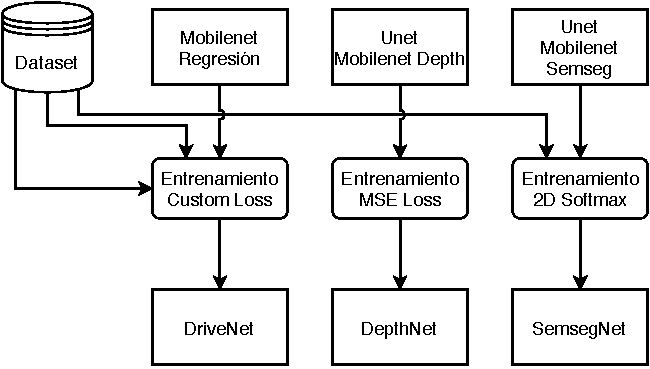
\includegraphics[scale=0.8]{imagenes/arquitectura_entrenamiento}
		\caption[Entrenamiento de tres redes neuronales]{entrenamiento de las tres redes neuronales}
		\label{training}
	\end{figure}
	
	Estos módulos están compuestos por tres redes neuronales basadas en la arquitectura Mobilenet V2, modificando la implementación estándar y su variante para inferencia de profundidad, un modelo estadístico llamado media exponencial móvil para el suavizado de la dirección, y el algoritmo K means para la cuantificación digital de colores.
	
	\subsection{RED DE CONDUCCIÓN}
		Denominada DriveNet, esta red es una modificación de la Mobilenet V2 estándar.
		
		\begin{figure}[H]
			\centering
			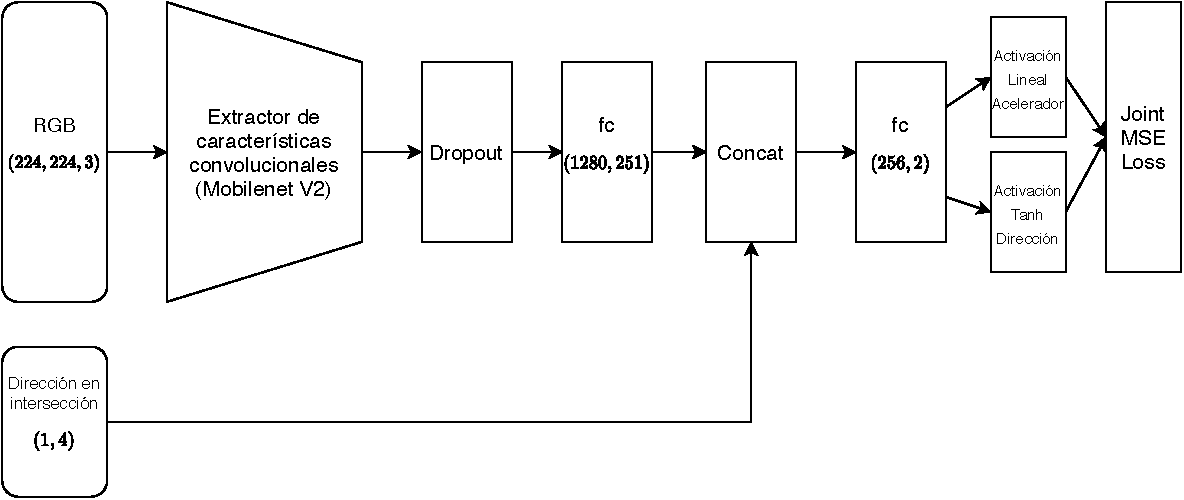
\includegraphics[scale=0.7]{imagenes/drivenet}
			\caption[Arquitectura DriveNet basada en Mobilenet V2]{Arquitectura DriveNet basada en Mobilenet V2}
			\label{drivenet}
		\end{figure}
	
		Se re define la sección del clasificador, en lugar de recibir los 1280 parámetros del extractor de características y predecir el número de clases, se convierte en una etapa de dos capas, una que recibe 1280 y exporta 251, a la que se le concatenan las 4 nuevas características, para enviar a la siguiente capa que recibirá 256 entradas y devuelve las 2 salidas finales, al adaptar la red a una tarea de regresión, el acelerador es un valor lineal entre 0 y 1, pero la dirección pasará por una tangente hiperbólica ($tanh(x)$) para mapear los valores entre $(-1, 1)$.
		
		\inputminted[frame=lines,
		baselinestretch=1,
		fontsize=\footnotesize,
		autogobble]{python}{codigos/marco-aplicativo/drivenet_capas.py}
		\captionof{listing}{definición de las capas de predicción}
		
		Como función de costo se usa el error cuadrático medio una para la aceleración y otra para la dirección, y la media de ambas como un costo conjunto denominado Joint MSE Loss.
		
		\inputminted[frame=lines,
		baselinestretch=1,
		fontsize=\footnotesize,
		autogobble]{python}{codigos/marco-aplicativo/drivenet_forward.py}
		\captionof{listing}{propagación hacia adelante y concatenación}
		
	\subsection{RED DE PROFUNDIDAD}
		Se usa la implementación de la red FastDepth sin modificaciones, basada en una MobilenetV2 con arquitectura de U-Net, los cambios que se dan son en la etapa de entrenamiento, ya que al ingresar las imágenes a la red, se trunca la distancia hasta máximo 30 metros, para simplificar la tarea de inferencia siendo que no es de interés centrarse en objetos a distancias mayores.
		
		\begin{figure}[H]
			\centering
			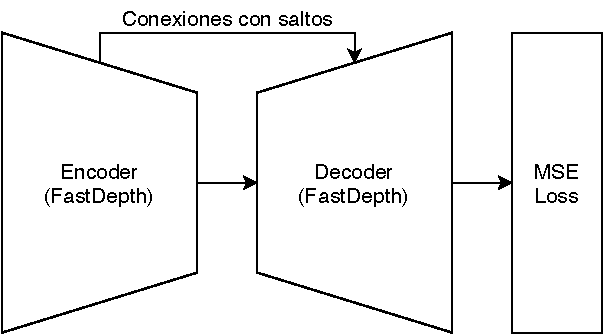
\includegraphics[scale=0.6]{imagenes/depthnet}
			\caption{Arquitectura FastDepth}
			\label{depthnet}
		\end{figure}
		
		\inputminted[frame=lines,
		baselinestretch=1,
		fontsize=\footnotesize,
		autogobble]{python}{codigos/marco-aplicativo/depthnet.py}
		\captionof{listing}{carga de la imagen para entrenamiento}
		
	\subsection{RED DE SEGMENTACIÓN SEMÁNTICA}
		Con el fin de simplificar las estructuras de los modelos, se utiliza la misma implementación de la red FastDepth modificando la función de costo por una Softmax 2D, ya que la tarea de segmentación semántica, es un tipo de clasificación píxel a píxel.
		
		\begin{figure}[H]
			\centering
			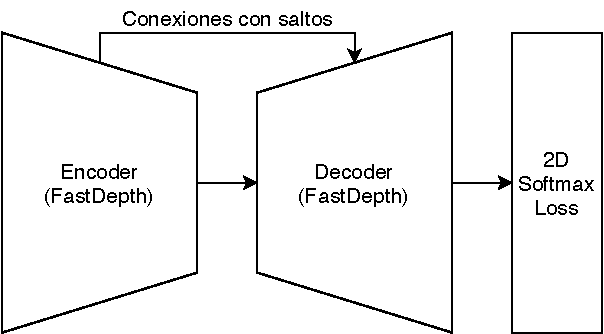
\includegraphics[scale=0.55]{imagenes/semsegnet}
			\caption{SemsegNet, FastDepth para clasificación 2D}
			\label{semsegnet}
		\end{figure}
		
	\subsection{SUAVIZADO DE DIRECCIÓN}
		Complementando las predicciones de las redes neuronales, se hace uso de una media exponencial móvil con parámetro $\alpha=0.7$, para suavizar las oscilaciones de la conducción con el fin de reducir ``volantazos'', tratando estos valores como una serie de tiempo.
		
		\begin{figure}[H]
			\centering
			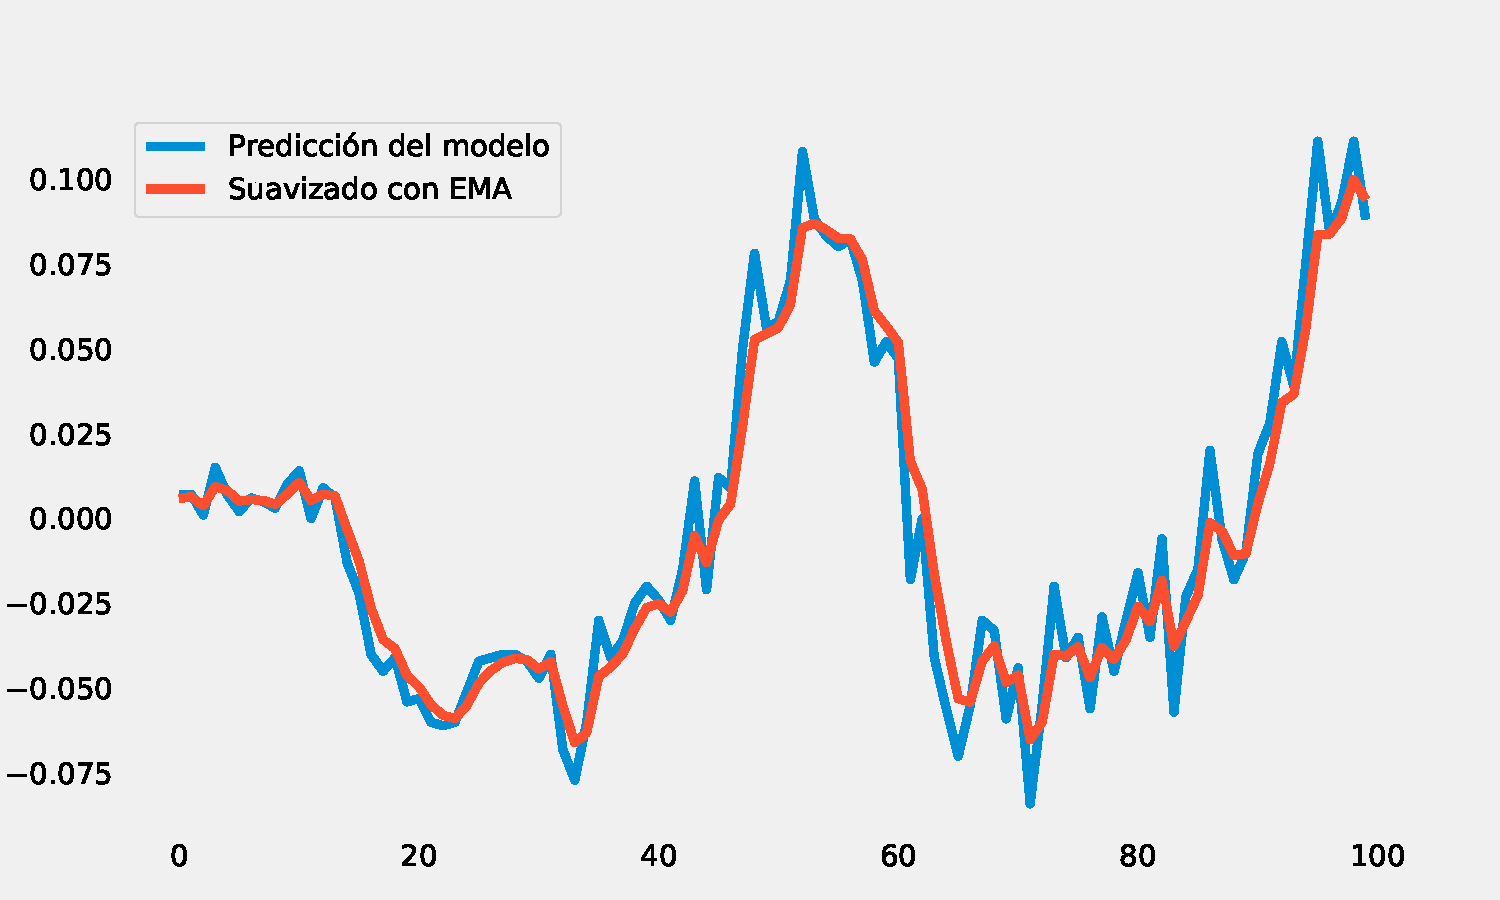
\includegraphics[scale=0.4]{imagenes/ema}
			\caption[Aplicación de medias exponenciales móviles]{Aplicación de medias exponenciales móviles para suavizar la dirección}
			\label{ema}
		\end{figure}
	
		Este modelo se aplica en cada iteración de la simulación a las predicciones de giro sólo cuando los valores están dentro del rango $(-0.2, 0.2)$ y fuera de una intersección, ya que valores mayores de giro indican que el vehículo está tomando una curva y no generando una oscilación.
		
		\inputminted[frame=lines,
		baselinestretch=1,
		fontsize=\footnotesize,
		autogobble]{python}{codigos/marco-aplicativo/ema.py}
		\captionof{listing}{uso de media exponencial móvil en la predicción}
		
	\subsection{CAJA DELIMITADORA}
		Una vez se tiene la máscara de píxeles que componen los semáforos luego de la limpieza por dilatación, erosión y apertura, se aplica el algoritmo Flood Fill de manera iterativa, partiendo por los píxeles a partir de la coordenada 120 en dirección horizontal, así cada vez que se encuentre un valor positivo de la máscara, el algoritmo lo ``pintará'' de ceros eliminando el objeto pero devolviendo las coordenadas de los puntos extremos arriba-izquierda y abajo-derecha que definen el rectángulo de mínima área delimitando el objeto.
		
		\inputminted[frame=lines,
		baselinestretch=1,
		fontsize=\footnotesize,
		autogobble]{python}{codigos/marco-aplicativo/flood_fill.py}
		\captionof{listing}{Flood Fill para la extracción de la caja delimitadora}
		
		Debido a que Python es un lenguaje interpretado y lento para tareas pesadas se compila la función mediante numba con el decorador @JIT (Just in Time Compilation).
		
	\subsection{CUANTIFICACIÓN DIGITAL DEL COLOR}
		Aplicando K-Means se reduce la cantidad de colores en la imagen, manteniendo los más predominantes, al ingresar al algoritmo un recorte que contiene específicamente un semáforo, los 4 colores más predominantes serán los de la luz emitida, de esta manera, se analiza la existencia de píxeles con valores mayores a cero en ciertos canales.
		
		\begin{figure}[H]
			\centering
			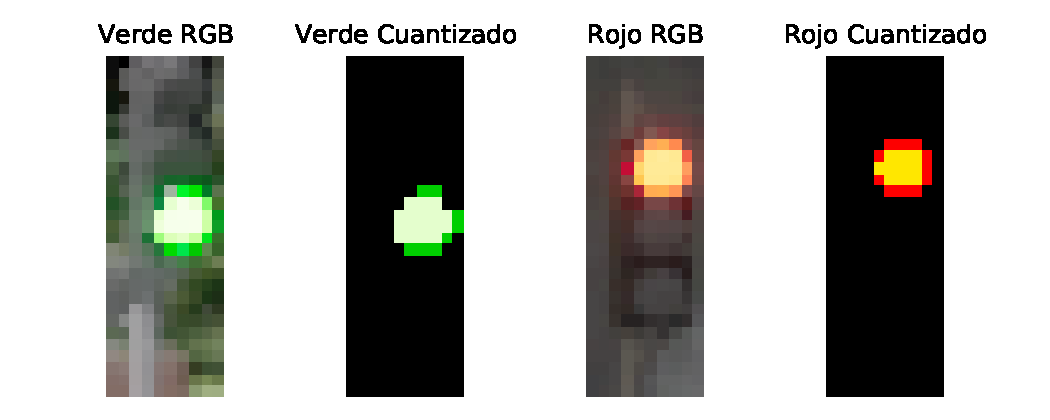
\includegraphics[scale=0.65]{imagenes/sign}
			\caption[Cuantificación digital del color]{cuantificación digital del color para clasificación de semáforos}
			\label{semaforo}
		\end{figure}
		
		En caso que los canales rojo o rojo y verde tengan valores distintos de cero, se tienen rojo o amarillo en cuyo caso el semáforo está en estado de pare, si los valores son positvos en verde y azúl, se tiene alguna tonalidad de verde o blanco como se observa en la figura \ref{semaforo}
		
		\inputminted[frame=lines,
		baselinestretch=1,
		fontsize=\footnotesize,
		autogobble]{python}{codigos/marco-aplicativo/kmeans.py}
		\captionof{listing}{kmeans para clasificación del color de semáforos}
				
	\subsection{MODELO PARA LA CONDUCCIÓN AUTÓNOMA}
		Una vez descritos todos los módulos, se define el modelo y sus interacciones.
		
		La entrada será una imagen en RGB de resolución $240\times180$, la cual pasará por las tres redes descritas.
		
		\begin{figure}[H]
			\centering
			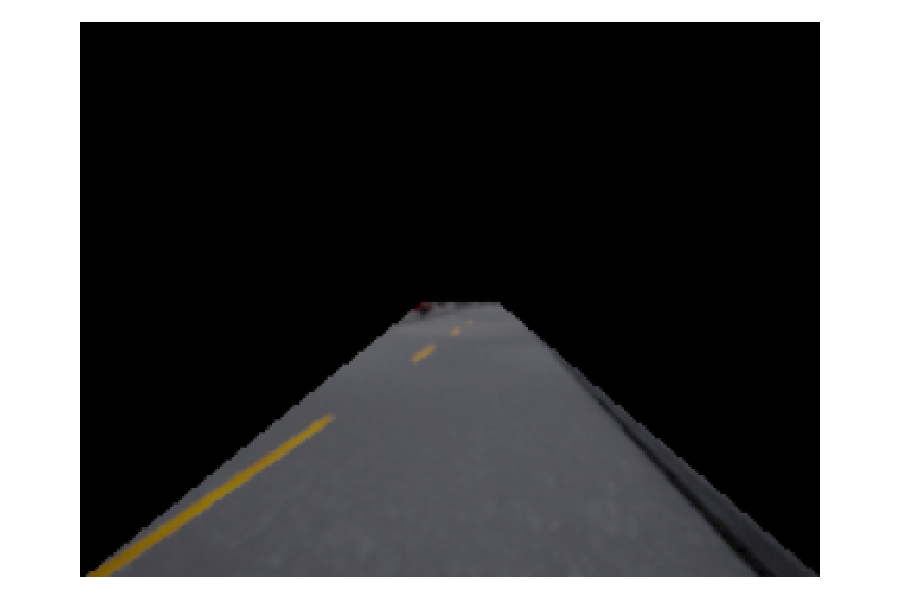
\includegraphics[scale=0.5]{imagenes/trapecio}
			\caption[Delimitado del área de interés para la detección de objetos]{trapecio delimitando el área de interés para la detección de obstáculos}
			\label{trapecio}
		\end{figure}
		
		Se usan las predicciones en conjunto de la DepthNet y SemsegNet, pasando previamente por una máscara que elimina todos los píxeles fuera de un trapecio (figura \ref{trapecio}) que corresponde al área de interés (con el fin de evitar falsos positivos), para extraer los píxeles correspondientes a posibles obstáculos, y se calcula la moda de las distancias redondeadas, para así decidir si existe peligro de colisión o no.
		
		\begin{figure}[H]
			\centering
			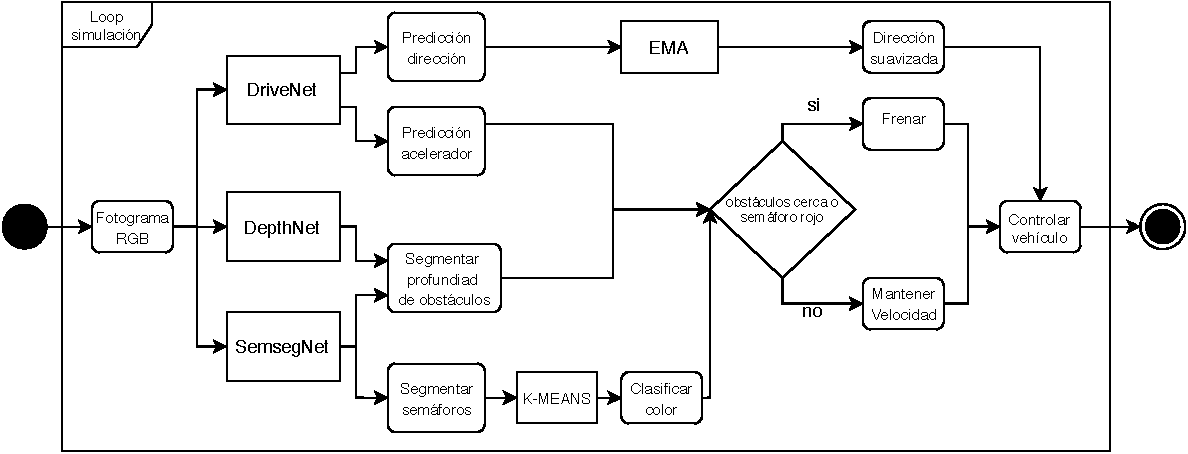
\includegraphics[scale=0.8]{imagenes/arquitectura_inferencia}
			\caption[Modelo de conducción autónoma]{modelo de conducción autónoma}
			\label{model}
		\end{figure}
		
		Se realiza un recorte a la zona donde se encuentre algún semáforo en caso de que se lo detecte, para lograr esta detección se aplica dilatación, erosión y apertura con el fin de reducir artefactos en las predicciones de la segmentación semántica, y se cuantiza el color para decidir si detenerse o no.
		
		Combinado con estas predicciones, la DriveNet infiere la dirección, la cual se suaviza mediante la media exponencial móvil, y aceleración, la cual se mantiene en caso de no presentarse obstáculos cerca ni semáforos en rojo.
		
		Los módulos descritos se pueden observar de manera estructurada en la figura \ref{model}.